\documentclass[10pt,hyperref={pdfpagemode=FullScreen},aspectratio=169]{beamer}

\usetheme[progressbar=frametitle]{metropolis}
\usepackage{appendixnumberbeamer}
\usepackage{lipsum}
\usepackage{amsmath}
\usepackage{amssymb}
\usepackage{booktabs}
\usepackage{siunitx}
\usepackage[scale=2]{ccicons}
\usepackage{pgfplots}
\usepgfplotslibrary{dateplot}
\usepackage{tikz}
\usetikzlibrary{positioning, shapes.geometric}
\pgfplotsset{compat=newest} % Allows to place the legend below plot
\usepgfplotslibrary{units} % Allows to enter the units nicely
\usepackage{circuitikz}
\usetikzlibrary{shapes,arrows}
\usepackage{dirtytalk}
\usepackage{xspace}




% Bibliography
\usepackage[
    backend=biber,
    style=ieee,
    natbib=true,
    url=false, 
    doi=true,
    eprint=false
]{biblatex}
%\addbibresource{references.bib}


\newcommand{\themename}{\textbf{\textsc{metropolis}}\xspace}
\newcommand{\universidade}{Universidade de Brasília}
\newcommand{\doctitle}{Princípios de Comunicação para Engenharia}

\definecolor{mpigreen}{HTML}{007977}
\setbeamercolor{frametitle}{bg=mpigreen}

\title{\doctitle}

\author{Daniel Araújo}
\institute{\universidade}
\titlegraphic{\hfill
\includegraphics[height=1.5cm]{../logo}}

\title{Introdução à Princípios de Comunicação}

\author{Prof. Daniel Costa Araújo}

\usepackage{graphicx}
\usepackage{subfigure}
\usepackage{verbatim}
\begin{document}


\frame{\titlepage}


\section{Conceitos Básicos}


\begin{frame}
  \frametitle{Sistemas Linear e Invariantes no Tempo}

  \begin{block}{Sistemas LTI podem ser bem caracterizados no tempo
    }
    $$y(t) = \int _{-\infty}^{\infty} h (t - \tau) x(\tau)d\tau$$

    em que, $h(t)$ é considerado o sistema, $x(t)$ é a entrada no mesmo e a saída do sistema é dado por $y(t)$ 
  \end{block}

\begin{block}{Sistemas LTI podem ser bem caracterizados na Frequencia}
  $$ Y(f) = H(f)X(f) $$

em que, 

\begin{align*}
   Y(f) = \mathcal{F}[y(t)] \\
   X(f) = \mathcal{F}[x(t)] \\
   H(f) = \mathcal{F}[h(t)] \\
\end{align*}

\end{block}

\end{frame}


\begin{frame}
  \frametitle{Transmissão}

Considerando o canal de transmissão como um sistema LIT é possível expressar o sinal recebido como:

  \begin{align*} 
  Y(f)   &= H(f)X(f) \\
  |Y(f)|e^{\jmath \theta _y(f)} &= |H(f)|e^{\jmath \theta _h(f)} |X(f)|e^{\jmath \theta _x(f)}
  \end{align*}
  Portanto,
  \begin{align*} 
  |Y(f)| &= |H(f)| |X(f)| \\
  \theta _y(f) &= \theta _h(f) + \theta _x(f)
  \end{align*}
  
  \begin{block}{NOTA}
    O sinal recebido é uma versão de $x(t)$ com  a amplitude e fase do sinal alteradas.
  \end{block}

\end{frame}


\section{Distorções em Transmissão}





\begin{frame}
  \frametitle{Transmissão sem distorção }

  \begin{block}{Quais as condições para que não haja distorção em uma transmissão? }
    O sinal recebido deve ser uma réplica do sinal transmitido. Ou seja, a forma de onda do sinal deve ser igual.
  
  
   - A condição de não-distorção é:
  
   $$
     y(t) = k x(t - t_d)
   $$
  
    - Representação na frequência: 
  
    $$
     Y(f) = k X(f)e^{-\jmath 2\pi f t_d}.
    $$
 
  \end{block}
\end{frame}

\begin{frame}
  \frametitle{Exemplo}

  \begin{columns}[T]
    \begin{column}{0.5\textwidth}
      \begin{figure}[!t]
        \begin{center}
          \begin{tikzpicture}
            \begin{axis}[
                width=0.9\textwidth, % Scale the plot to \linewidth
                grid = major, % Display a grid
                grid style={dashed,gray!30}, % Set the style
                xlabel= Frequência, % Set the labels
                ylabel= Amplitude,
                ymin=-3.5, ymax=3.5,
                xmin = -400, xmax = 400,
                x unit=\si{\hertz}, % Set the respective units
                legend style={at={(0,1)},anchor=south west}, % Put the legend below the plot
                %x tick label style={rotate=90,anchor=east} % Display labels sideways
              ]
              
            
              \addplot+ [no marks]
              table[x=Frequencia,y=Amplitude,col sep=comma] {Fig/chan_ideal.csv}; 
              
              \addplot+ [no marks,red, dashed]
              table[x=Frequencia,y=Fase,col sep=comma] {Fig/chan_ideal.csv};
    
              \legend{Amplitude,Fase}
            \end{axis}
          \end{tikzpicture}
          \caption{Representação de um canal sem distorção.}
        \end{center}
      \end{figure}

    \end{column}
    \begin{column}{0.5\textwidth
      }
      \begin{block}{Análise em frequência}
        $$
         H(f) = k e^{-\jmath 2\pi f t_d}
         $$
         
         \begin{itemize}
          \item Frequência angular : $\omega = 2\pi f$
          \item Atraso de grupo : $t_d = - \frac{1}{2\pi}\frac{d \theta(f)}{df}$ 
          \item Atraso de portadora : $t_p = -\frac{\theta(f_0)}{2\pi f_o}$ 
         \end{itemize}
        
        \end{block}
        \begin{block}{Sistemas passa-tudo são sempre canais sem distoção?}
          \begin{itemize}
            \item Não. Sistemas passa-tudo não implica em fase linear. 
   
            \item É possível termos sistemas passa-tudo com fase não-linear.
          \end{itemize}
        \end{block}
    \end{column}
  \end{columns}

\end{frame}


\begin{frame}
  \frametitle{Exemplo}

  \begin{block}{Filtro}
    Considere um filtro RC passa-baixa com $R=10^3$ e $C = 10^{-9}$, cuja a entrada e a saída são $g(t)$ e $y(t)$, respectivamente. Determine a função de transferência $H(f)$, a fase e o atraso de grupo. Considere que para um transmissão sem distorção o requisito é que a amplitude na saída esteja dentro de 2\% e que o atraso de grupo esteja dentro 5\% de variação.
  \end{block}

\end{frame}

\begin{frame}
  \frametitle{Solução}

  
\begin{align*}
H(f) &= \frac{1/(\jmath 2\pi fC)}{R + 1/(\jmath 2\pi fC)} \\
    & = \frac{1}{1 + \jmath 2\pi f RC } \\
    & = \frac{a}{a+ \jmath 2\pi f }
\end{align*}


em que $a = \frac{1}{RC} = 10 ^6$ 

Então:


\begin{align*}
|H(f)| & = \frac{a}{\sqrt{a ^2+  (2\pi f)^2 }} \approx 1, \,\ |2\pi f| << a \\
\theta _h (f) &= - \arctan {\frac{2\pi f}{a}} \approx \frac{2\pi f}{a}, \,\ |2\pi f| << a 
\end{align*}

\end{frame}


\begin{frame}
  \frametitle{Solução: continuação}


\begin{columns}[T]

  
  \begin{column}{0.5\textwidth}
    Para acharmos o atraso de grupo basta derivar o $\theta _h (f)$: 

    \begin{align*}
    t_d(f) &= -\frac{1}{2\pi}\frac{\partial }{\partial f}\theta _h (f)  \\
       & =  \frac{a}{a^2 +( 2\pi f)^2 } \\ 
       & \approx \frac{1}{a} , \,\ |2\pi f| << a   \\
       & \approx 10^{-6}
    \end{align*}
    
    
    Para calcular a banda efetiva basta considerarmos $|H(B)|> 0.98$ e $t_d(B)> 0.95/a$
    
  \end{column}
  \begin{column}{0.5\textwidth}
    $$
|H(f)|  = \frac{a}{\sqrt{a ^2+  (2\pi f)^2 }} \geq 0.98
$$
e
$$
t_d(f)  = \frac{a}{a^2 +( 2\pi f)^2}  \geq \frac{0.95}{a}
$$

A menor frequência que atende as duas equações é $B=32.31$ \si{\kilo\hertz}
  \end{column}
\end{columns}
\end{frame}


\begin{frame}
  \frametitle{Representação do filtro}

  \begin{figure}[!t]
    \begin{center}
      \begin{tikzpicture}
        \begin{semilogxaxis}[
            width=0.65\textwidth, % Scale the plot to \linewidth
            grid = major, % Display a grid
            grid style={dashed,gray!30}, % Set the style
            xlabel= Frequência, % Set the labels
            ylabel= Amplitude,
            ymin=-1.5, ymax=0,
            xmin = 100, xmax = 100000,
            x unit=\si{\hertz}, % Set the respective units
            legend style={at={(0,0)},anchor=south west}, % Put the legend below the plot
            %x tick label style={rotate=90,anchor=east} % Display labels sideways
          ]
                  
          \addplot+ [no marks,line width=2pt]
          table[x=Frequencia,y=FaseFiltro,col sep=comma] {Fig/filter_model.csv}; 

          \addplot+ [no marks,black, dashed,line width=2pt]
          table[x=Frequencia,y=Approx,col sep=comma] {Fig/filter_model.csv};

          \addplot+ [no marks,green, dashed,line width=2pt]
          table[x=Frequencia2,y=Banda,col sep=comma] {Fig/filter_model.csv};
          
          \legend{Fase do filtro,Aproximação,Largura de Banda s/ distorção}
        \end{semilogxaxis}
      \end{tikzpicture}
      \caption{Modelo em Filtro Passa-baixa.}
    \end{center}
  \end{figure}

\end{frame}

\section{Tipos de Distorções}

\begin{frame}
  \frametitle{Distorção linear}
\begin{itemize}
  \item Causado por um espalhamento temporal do sinal como mostrado nas figuras
  \item No exemplo a seguir, a relação de entrada e saída  é expressa por
  $$
   y(t) = x(t-t_d) + \frac{k}{2}\left[x(t-t_d - T/2) + x(t-t_d - T)\right]
  $$
  \item Pela expressão, é possível perceber que o é espalhado ao longo do tempo, efeito corroborado pelos gráficos
\end{itemize}
  

\end{frame}


\begin{frame}
  \frametitle{Distorções não-lineares}

  Em certos casos, efeitos não-lineares estão integrados em canais de comunicação.

  \begin{itemize}
    \item A relação de entrada-saída é escrita como:
    $$
    y(t) = f(x(t)),
    $$ 
    em que $f(.)$ consiste em um função de mapeamento não-linear
    
    \item  Neste casos, podemos reescrever o problem em termos da série de Maclaurin
    $$
    y(t) = a_0 + a_1x(t)+ a_2x^2(t) + ...
    $$
  \end{itemize}


\end{frame}

\begin{frame}
  \frametitle{Exemplo}

  \begin{columns}
    \begin{column}{0.45\textwidth}
      


      \begin{figure}[!t]
        \begin{center}
          \begin{tikzpicture}
            \begin{axis}[
                width=\textwidth, % Scale the plot to \linewidth
                grid = major, % Display a grid
                grid style={dashed,gray!30}, % Set the style
                xlabel= Frequência, % Set the labels
                ylabel= Amplitude,
                ymin=-0.2, ymax=1,
                xmin = 0, xmax = 1,
                x unit=\si{\second}, % Set the respective units
                legend style={at={(0,1)},anchor=south west}, % Put the legend below the plot
                %x tick label style={rotate=90,anchor=east} % Display labels sideways
              ]
              
            
              \addplot+ [no marks,line width=2pt]
              table[x=Tempo,y=x,col sep=comma] {Fig/nonlinchan.csv}; 
              
              \addplot+ [no marks,red, dashed,line width=2pt]
              table[x=Tempo,y=y,col sep=comma] {Fig/nonlinchan.csv};
    
              \legend{Sinal de entrada,Sinal de saída}
            \end{axis}
          \end{tikzpicture}
          \caption{Representação no tempo.}
        \end{center}
      \end{figure}




    \end{column}



    \begin{column}{0.45\textwidth}
      

        \begin{figure}[!t]
          \begin{center}
            \begin{tikzpicture}
              \begin{axis}[
                  width=\textwidth, % Scale the plot to \linewidth
                  grid = major, % Display a grid
                  grid style={dashed,gray!30}, % Set the style
                  xlabel= Tempo, % Set the labels
                  ylabel= Amplitude,
                  ymin=0, ymax=5,
                  xmin = -100, xmax = 100,
                  x unit=\si{\hertz}, % Set the respective units
                  legend style={at={(0,1)},anchor=south west}, % Put the legend below the plot
                  %x tick label style={rotate=90,anchor=east} % Display labels sideways
                ]
                
              
                \addplot+ [no marks,line width=2pt]
                table[x=Frequencia,y=Xf,col sep=comma] {Fig/nonlinchan.csv}; 
                
                \addplot+ [no marks,red, dashed,line width=2pt]
                table[x=Frequencia,y=Yf,col sep=comma] {Fig/nonlinchan.csv};
      
                \legend{Sinal de entrada,Sinal de saída}
              \end{axis}
            \end{tikzpicture}
            \caption{Representação no frequência.}
          \end{center}
        \end{figure}


    \end{column}


  \end{columns}


\end{frame}


\begin{frame}
  \frametitle{ Distorção de multi-percurso}

  \begin{block}{Modelo de canal}
    $$
h(t) = \sum _{i=0}^{N-1}k_i \delta (t - \tau _i),
$$

em que $k_i$ é atenuação correspondente ao $i$-ésimo multi percurso e $\tau _i$ é atraso relativo ao $i$-ésimo multi percurso.

  \end{block}

  \begin{figure}[!h]
    \centering
    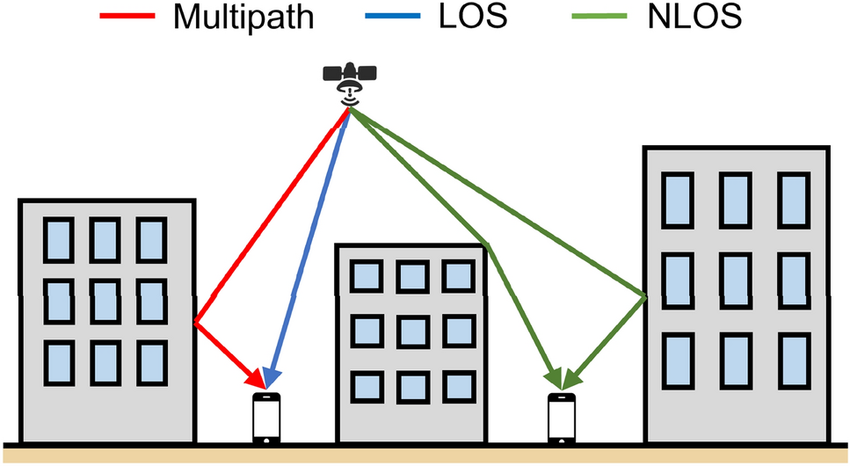
\includegraphics[width=0.5\textwidth]{Fig/multipath_channel.png}
  \end{figure}

\end{frame}

\section{Sinais do Tipo Energia e Potência}


\begin{frame}
  \frametitle{ Definição }

   A energia de um sinal $x(t)$ é dado por 
  
  $$
  E_x = \int _{-\infty}^{\infty} |x(t)|^2 dt
  $$
  Um sinal é chamado do tipo energia se $E_g$ possui convergência.
\end{frame}


\begin{frame}
  \frametitle{Energia em função da frequência}

\begin{columns}[T]
  \begin{column}{0.5\textwidth}
    \begin{block}{Como definir o a energia no domínio da frequência?
      }
      \begin{align*}
        E_x & = \int _{-\infty}^{\infty} |x(t)|^2 dt \\
            & = \int _{-\infty}^{\infty} x(t)x^*(t) dt \\
            & = \int  _{-\infty}^{\infty} x(t) \left[  \int  _{-\infty}^{\infty}X^*(f) e^{-\jmath 2 \pi f t} df \right] dt \\
            & = \int  _{-\infty}^{\infty} X^*(f) \left[  \int  _{-\infty}^{\infty}x(t)  e^{-\jmath 2 \pi f t} dt \right] df \\
            & = \int  _{-\infty}^{\infty} X^*(f) X(f) df \\
            & = \int  _{-\infty}^{\infty} |X(f)|^2 df 
        \end{align*}
        
    \end{block}
    
  \end{column}
  \begin{column}{0.5\textwidth}
    \begin{block}{Teorema de Parseval}
      $$ E_x = \int _{-\infty}^{\infty} |x(t)|^2 dt = \int  _{-\infty}^{\infty} |X(f)|^2 df $$
    \end{block}

  \end{column}
\end{columns}

\end{frame}

\begin{frame}
  \frametitle{Exemplo}

  Considere o o sinal $g(t) = e^{-at} u(t)$, em que $u(t)$ é uma função degrau. Calcule a energia do sinal $x(t)$ pela definição no tempo e na frequência

\end{frame}


\begin{frame}
  \frametitle{Solução: Análise no tempo}

  \begin{align*}
    E_g & = \int _{0}^{\infty} e^{-2at} dt \\
        & = - \frac{1}{2a} e^{-2at} \Biggr|_{0}^{\infty} \\
        & =  - \frac{1}{2a} \left[ \lim _{t \rightarrow \infty}e^{-2at} - e^{-2a0}\right]  \\
        & =  - \frac{1}{2a} \left[ 0 - 1\right]  \\
        & =  \frac{1}{2a}
    \end{align*}
    

\end{frame}

\begin{frame}
  \frametitle{Solução: Análise na frequência}
  

  \begin{columns}[T]

    \begin{column}{0.5\textwidth}
      
        
    \begin{block}{Sinal em frequência}
      \begin{align*}
        G(f) & = \int _{0}^{\infty}x(t) e^{-\jmath 2 \pi ft} dt \\
             &=  \frac{1}{a + \jmath 2 \pi f}
        \end{align*}
        
        
        
        \begin{align*}
        |G(f)|^2 &=  \frac{1}{a^2 + (2 \pi f)^2}
        \end{align*}
        
    \end{block}
    \end{column}
    \begin{column}{0.5\textwidth}
      \begin{block}{Cálculo da energia}
        \begin{align*}
          E_g & = \int _{-\infty}^{\infty} \frac{1}{a^2 + (2 \pi f)^2} df \\ 
              & = \frac{1}{a^2}\int _{-\infty}^{\infty} \frac{1}{1 + \left(\frac{2 \pi f}{a}\right)^2} df \\
              & = \frac{1}{a^2}\int _{-\infty}^{\infty} \frac{1}{1 + \left(u\right)^2} \left(\frac{a}{2\pi}\right) du\\
              & = \frac{1}{2\pi a}\int _{-\infty}^{\infty} \frac{1}{1 + u^2} du\\
              & = \frac{1}{2\pi a} atan \left(\frac{2 \pi f}{a} \right)\Biggr|_{-\infty}^{\infty} \\
              & = \frac{1}{2\pi a} \left[\frac{ \pi }{2} - \frac{- \pi }{2}  \right] = \frac{1}{2 a}
          \end{align*}
      \end{block}
    \end{column}
  \end{columns}
    

\end{frame}

\section{Classificação quanto a Banda}

\begin{frame}
  \frametitle{Banda efetiva}

  \begin{block}{Definição}
    Corresponde a porção positiva da frequência ($f>0$) na qual o sinal é diferente de zero.
  \end{block}

  \begin{itemize}
    \item Sinais limitados no tempo geram sinais não-limitados na frequência (Veja exemplo a seguir)
    \item A banda é definida segundo o percentual de energia considerado como limiar
    \begin{itemize}
      \item  Exemplo: Considerando 90 \% da energia total é possível obter uma banda correspondente. Para o exemplo da figura isso seria em torno de $B = \frac{1}{\pi}$ \si{\hertz}
    \end{itemize}
  \end{itemize}

\end{frame}



\begin{frame}
  \frametitle{Representação}


  \begin{columns}
    \begin{column}{0.5\textwidth}
      
      \begin{figure}[!t]
        \begin{center}
          \begin{tikzpicture}
            \begin{axis}[
                width=\textwidth, % Scale the plot to \linewidth
                grid = major, % Display a grid
                grid style={dashed,gray!30}, % Set the style
                xlabel= Tempo, % Set the labels
                ylabel= Amplitude,
                ymin=0, ymax=1.2,
                xmin = -20, xmax = 20,
                x unit=\si{\hertz}, % Set the respective units
                legend style={at={(0,1)},anchor=south west}, % Put the legend below the plot
                %x tick label style={rotate=90,anchor=east} % Display labels sideways
              ]
              
            
              \addplot+ [no marks,line width=0.1pt]
              table[x=Tempo,y=m,col sep=comma] {Fig/sinal_rect.csv}; 
            
    
              \legend{Sinal no Tempo}
            \end{axis}
          \end{tikzpicture}
          \caption{Representação no Tempo.}
        \end{center}
      \end{figure}



    \end{column}

    \begin{column}{0.5\textwidth}
      
      \begin{figure}[!t]
        \begin{center}
          \begin{tikzpicture}
            \begin{axis}[
                width=\textwidth, % Scale the plot to \linewidth
                grid = major, % Display a grid
                grid style={dashed,gray!30}, % Set the style
                xlabel= Frequência, % Set the labels
                ylabel= Amplitude,
                ymin=0, ymax=1,
                xmin = -2, xmax = 2,
                x unit=\si{\hertz}, % Set the respective units
                legend style={at={(0,1)},anchor=south west}, % Put the legend below the plot
                %x tick label style={rotate=90,anchor=east} % Display labels sideways
              ]
              
            
              \addplot+ [no marks,line width=0.1pt]
              table[x=Frequencia,y=Mf,col sep=comma] {Fig/sinal_rect.csv}; 
            
    
              \legend{Sinal em Frequência}
            \end{axis}
          \end{tikzpicture}
          \caption{Representação no frequência.}
        \end{center}
      \end{figure}

    \end{column}
  \end{columns}

  

\end{frame}

\begin{frame}
  \frametitle{Sinais do tipo Potência}

  A energia de um sinal $x(t)$ é um algun problemas não converge:

$$
E_x = \int _{-\infty}^{\infty} |x(t)|^2 dt \rightarrow \infty
$$
Neste caso, é utilizado o conceito de potência

$$
P_x = \lim _{T \rightarrow \infty} \frac{1}{T}\int _{-T/2}^{T/2} |x(t)|^2 dt,
$$

o qual consiste em um média da energia ao longo do tempo.


Os resultados anteriores podem ser reescrito em função da frequência portanto é possível:
\begin{itemize}
  \item  usar o teorema de Parseval para a potência
  \item usar a banda efetiva em termos da potência
\end{itemize}

\end{frame}

\section{Representação em Banda Básica e Banda Passante}

\begin{frame}
  \frametitle{Definição}

  \begin{block}{Conceito}
    São sinais cujo espectro estão centrados na frequência 0.

  \end{block}

  \begin{block}{Exemplos}
    \begin{itemize}
      \item Música 
      \item Voz
      \item Vídeo
    
    \end{itemize}
  \end{block}
\end{frame}


\begin{frame}
  \frametitle{Exemplo de sinal em Banda-básica}


  \begin{columns}
    \begin{column}{0.5\textwidth}
      
      \begin{figure}[!t]
        \begin{center}
          \begin{tikzpicture}
            \begin{axis}[
                width=\textwidth, % Scale the plot to \linewidth
                grid = major, % Display a grid
                grid style={dashed,gray!30}, % Set the style
                xlabel= Tempo, % Set the labels
                ylabel= Amplitude,
                ymin=0, ymax=1.2,
                xmin = -20, xmax = 20,
                x unit=\si{\hertz}, % Set the respective units
                legend style={at={(0,1)},anchor=south west}, % Put the legend below the plot
                %x tick label style={rotate=90,anchor=east} % Display labels sideways
              ]
              
            
              \addplot+ [no marks,line width=0.1pt]
              table[x=Tempo,y=m,col sep=comma] {Fig/sinal_rect.csv}; 
            
    
              \legend{Sinal no Tempo}
            \end{axis}
          \end{tikzpicture}
          \caption{Representação no Tempo.}
        \end{center}
      \end{figure}



    \end{column}

    \begin{column}{0.5\textwidth}
      
      \begin{figure}[!t]
        \begin{center}
          \begin{tikzpicture}
            \begin{axis}[
                width=\textwidth, % Scale the plot to \linewidth
                grid = major, % Display a grid
                grid style={dashed,gray!30}, % Set the style
                xlabel= Frequência, % Set the labels
                ylabel= Amplitude,
                ymin=0, ymax=1,
                xmin = -2, xmax = 2,
                x unit=\si{\hertz}, % Set the respective units
                legend style={at={(0,1)},anchor=south west}, % Put the legend below the plot
                %x tick label style={rotate=90,anchor=east} % Display labels sideways
              ]
              
            
              \addplot+ [no marks,line width=0.1pt]
              table[x=Frequencia,y=Mf,col sep=comma] {Fig/sinal_rect.csv}; 
            
    
              \legend{Sinal em Frequência}
            \end{axis}
          \end{tikzpicture}
          \caption{Representação na frequência.}
        \end{center}
      \end{figure}

    \end{column}
  \end{columns}
\end{frame}


\begin{frame}
  \frametitle{Exemplo de sinal em Banda-Passante}


  \begin{columns}
    \begin{column}{0.5\textwidth}
      
      \begin{figure}[!t]
        \begin{center}
          \begin{tikzpicture}
            \begin{axis}[
                width=\textwidth, % Scale the plot to \linewidth
                grid = major, % Display a grid
                grid style={dashed,gray!30}, % Set the style
                xlabel= Tempo, % Set the labels
                ylabel= Amplitude,
                ymin=-1.2, ymax=1.2,
                xmin = -20, xmax = 20,
                x unit=\si{\second}, % Set the respective units
                legend style={at={(0,1)},anchor=south west}, % Put the legend below the plot
                %x tick label style={rotate=90,anchor=east} % Display labels sideways
              ]
              
            
              \addplot+ [no marks,line width=0.1pt]
              table[x=Tempo,y=m,col sep=comma] {Fig/passband.csv}; 
            
    
              \legend{Sinal no Tempo}
            \end{axis}
          \end{tikzpicture}
          \caption{Representação no Tempo.}
        \end{center}
      \end{figure}



    \end{column}

    \begin{column}{0.5\textwidth}
      
      \begin{figure}[!t]
        \begin{center}
          \begin{tikzpicture}
            \begin{axis}[
                width=\textwidth, % Scale the plot to \linewidth
                grid = major, % Display a grid
                grid style={dashed,gray!30}, % Set the style
                xlabel= Frequência, % Set the labels
                ylabel= Amplitude,
                ymin=0, ymax=1,
                xmin = -10, xmax = 10,
                x unit=\si{\hertz}, % Set the respective units
                legend style={at={(0,1)},anchor=south west}, % Put the legend below the plot
                %x tick label style={rotate=90,anchor=east} % Display labels sideways
              ]
              
            
              \addplot+ [no marks,line width=0.1pt]
              table[x=Frequencia,y=Mf,col sep=comma] {Fig/passband.csv}; 
            
    
              \legend{Sinal em Frequência}
            \end{axis}
          \end{tikzpicture}
          \caption{Representação na frequência.}
        \end{center}
      \end{figure}

    \end{column}
  \end{columns}


\end{frame}

\subsection{Conversão de Banda-básica para Banda-passante}

\begin{frame}
  \frametitle{Equivalente de banda-básica}

  Considere a seguinte definição 
  \begin{align*}
  x_+(t) &=  \mathcal{F}^{-1}[X_+(f)] \\
         &=  \mathcal{F}^{-1}[X(f)u(f)] \\
         &=  x(t) \circ (\frac{1}{2} \delta (t) + \jmath \frac{1}{2\pi t}) \\
         &=  \frac{1}{2}x(t) + \jmath \frac{1}{2}\hat{x}(t)
  \end{align*}
  
  
  em que 
  
  $$ 
   \mathcal{F}[\hat{x}(t)] = -\jmath \textrm{sgn}(f)X(f)
  $$
  ou seja o filtro de Hilbert é dado por
  
  $$
  \mathcal{F}[\frac{1}{\pi t}]  =  -\jmath \textrm{sgn}(f)
  $$
  

\end{frame}

\begin{frame}
  \frametitle{Entendo a transformada de Hilbert
  }
  Considere o sinal $m(t) = \cos \left(2\pi f_m t\right)$. Calcule a sua transformada de hilbert.

  Primeiramente vamos converter o sinal para frequência:
    $$
    M(f) = \frac{1}{2}\left(\delta (f - f_m) + \delta (f + f_m) \right)
    $$
  
    
    \begin{align*}
      \mathcal{F}[\hat{m}(t)] & = -\jmath \textrm{sgn}(f)M(f) \\
                              & = -\jmath \textrm{sgn}(f)\left(\frac{1}{2}\left(\delta (f - f_m) + \delta (f + f_m) \right)\right)\\
                              & = -\frac{\jmath}{2} \left( \delta (f - f_m)  -  \delta (f + f_m)  \right) \\
                              & =  \frac{1}{2\jmath} \left( \delta (f - f_m)  -  \delta (f + f_m)  \right)
    \end{align*}  
  

\end{frame}


\begin{frame}
  \frametitle{Filtro defasador}

  \begin{columns}
    \begin{column}{0.5\textwidth
      }
      Portanto, 
  
  $$
  \hat{m}(t)  =  \sin \left(2\pi f_m t\right)
  $$
  
  \begin{block}{IMPROTANTE}
    A transformada de Hilbert é um filtro defasador.
  \end{block}
    \end{column}
    \begin{column}{0.5\textwidth}

      \begin{figure}[!t]
        \begin{center}
          \begin{tikzpicture}
            \begin{axis}[
                width=\textwidth, % Scale the plot to \linewidth
                grid = major, % Display a grid
                grid style={dashed,gray!30}, % Set the style
                xlabel= Tempo, % Set the labels
                ylabel= Amplitude,
                ymin=-1.2, ymax=1.2,
                xmin = 0, xmax = 20,
                x unit=\si{\second}, % Set the respective units
                legend style={at={(0,1)},anchor=south west}, % Put the legend below the plot
                %x tick label style={rotate=90,anchor=east} % Display labels sideways
              ]
              
            
              \addplot+ [no marks,line width=0.1pt]
              table[x=Tempo,y=m,col sep=comma] {Fig/hilbert.csv}; 
              \addplot+ [no marks,red,line width=0.1pt]
              table[x=Tempo,y=hat_m,col sep=comma] {Fig/hilbert.csv};
            
    
              \legend{$m(t)$,$\hat{m}(t)$}
            \end{axis}
          \end{tikzpicture}
          \caption{Representação no Tempo.}
        \end{center}
      \end{figure}
      
    \end{column}
  \end{columns}
  
  
\end{frame}

\begin{frame}
  \frametitle{Equivalente passa-baixa}

  \begin{block}{Defnição
    }
    O equivalente passa-baixa de um sinal $x(t)$ é dado por
    $$
    X_l(f) = 2X_+(f+f_o) \newline
    = 2X(f+f_o) U(f + f_o)
$$
  \end{block}




Convertendo para o tempo:

$$
  x_l(t) =\mathcal{F}^{-1}[X_l(f)] \newline
         = 2x_+(t)e^{-\jmath 2 \pi f_o t} \newline
         = (x(t) + \jmath \hat {x}(t))e^{-\jmath 2 \pi f_o t}.
$$
Portanto:

$$
  x(t) = Re\{ x_l(t)e^{\jmath 2 \pi f_o t}\}
$$


\end{frame}


\begin{frame}
  \frametitle{Componentes em fase e quadratura}

  Componentes em fase e quadratura


\begin{align*}
   x_l(t) &= (x(t) + \jmath \hat {x}(t))e^{-\jmath 2 \pi f_o t} \\
          &= (x(t)\cos(2\pi f_o t) + \hat {x}(t)\sin(2 \pi f_o t) ) + \jmath (\hat {x}(t)\cos(2\pi f_o t) - x(t)\sin(2 \pi f_o t) )
\end{align*}

A componente real é chamada de fase:
$$
   x_i(t) = x(t)\cos(2\pi f_o t) + \hat {x}(t)\sin(2 \pi f_o t)
$$

A componente imaginária é chamada de quadratura:
$$
  x_q(t) = \hat {x}(t)\cos(2\pi f_o t) - x(t)\sin(2 \pi f_o t)
$$

\end{frame}


\begin{frame}
  \frametitle{Representação Matricial}

  Das duas expressões é possível escrevê-las de forma matricial :
$$
\begin{bmatrix} x_i(t)  \\ x_q(t) \end{bmatrix} = \begin{bmatrix} \cos(2\pi f_o t) & \sin(2 \pi f_o t)  \\ -\sin(2 \pi f_o t)  & \cos(2\pi f_o t)\end{bmatrix} \begin{bmatrix} x(t)  \\ \hat {x}(t) \end{bmatrix}
$$

\begin{block}{Receptor}
  A expressão define a operação de recepção. Indica a converssão do sinal de banda-passante para o seu equivalente passa-baixa
\end{block}


A expreesão inversa pode ser obtida através da inversão matricial. 

$$
\begin{bmatrix} x(t)  \\ \hat {x}(t) \end{bmatrix} = \begin{bmatrix} \cos(2\pi f_o t) & -\sin(2 \pi f_o t)  \\ \sin(2 \pi f_o t)  & \cos(2\pi f_o t)\end{bmatrix} \begin{bmatrix}  x_i(t)  \\ x_q(t) \end{bmatrix}
$$

\begin{block}{Transmissor}
  A expressão define a operação de transmissão. Indica a conversão do sinal de banda-básica para a banda passante
\end{block}

\end{frame}

\begin{frame}
  \frametitle{ Representação Cartesiana x Polar}


  \begin{columns}[T]
    \begin{column}{0.5\textwidth}
      \begin{block}{Representação cartesiana}
        $$
        x_l(t) = x_i(t) + \jmath x_q(t)
       $$
       \end{block}
     
       \begin{block}{Representação polar}
         $$
      x_l(t) = r(t) e^{\jmath \theta}
      $$
      em que 
      $$
      r(t) = \sqrt{x^2_i(t) + x^2_q(t)}
      $$
      e
      $$
      \theta (t) = \textrm{arctan}{\left( \frac{x_q(t)}{x_i(t)} \right)}
      $$
       \end{block}
    \end{column}
    \begin{column}{0.5\textwidth}
      \begin{block}{Sinal de banda-passante}
        $$
    x(t) = Re\{r(t)e^{\jmath 2\pi f_o t + \theta}\}
    $$
    $$
    x(t)  =  r(t)\cos(2\pi f_o t + \theta)
    $$
      \end{block}

      \begin{block}{IMPROTANTE}
        O sinal $r(t)$ é denominado como envelope complexo.
        
      \end{block}
    \end{column}
    \end{columns}

  

  
\end{frame}


\begin{frame}
  \frametitle{Considerações sobre energia}

  \begin{columns}[T]
    \begin{column}{0.5\textwidth}
      \begin{itemize}
        \item Pelo teorema de Parseval 
        $$
      E_x = \int _{-\infty}^{\infty} |x(t)|^2 dt  =  \int _{-\infty}^{\infty} |X(f)|^2 df  
      $$
      \item A energia de banda-básica e banda-passante é dado por:
      \begin{align*}
        E_x &= \int _{-\infty}^{\infty}  | X_+(f) + X_-(f)|^2 df \\ 
            &=  \int _{-\infty}^{\infty}  | X_+(f)|^2 df + \int _{-\infty}^{\infty}  | X_-(f)|^2 df \\
            &= 2\int _{-\infty}^{\infty}  | X_+(f)|^2 df \\
            &= 2 E_{x_+}
        \end{align*}
      \end{itemize}
      
    \end{column}
    \begin{column}{0.5\textwidth}
    \begin{itemize}
      \item  Utilizando a representação de banda-básica tem-se que 
       \begin{align*}
       E_x &= 2 E_{x_+}  \\
          &= \int _{-\infty}^{\infty}  | X_+(f)|^2 df \\
          &= 2 \int _{-\infty}^{\infty}  | \frac{X_l(f)}{2}|^2 df \\
          &= \frac{2}{4} \int _{-\infty}^{\infty}  | X_l(f)|^2 df \\
          &= \frac{1}{2}\int _{-\infty}^{\infty}  | X_l(f)|^2 df  \\
          &= \frac{1}{2} E_{x_l}
       \end{align*}
      
    \end{itemize}

    \end{column}
    \end{columns}
    {
      \begin{block}{IMPROTANTE}
        Energia da banda passante é metade da energia de banda-básica.
      \end{block}}
\end{frame}


\end{document}